%-----------------------------------------
\begin{frame}
\frametitle{Coastal waveguide view}
\begin{columns}
    \begin{column}{0.5\textwidth}
      \centering
      framework for aggregation\\
      targeted evaluation \\
      guidance and `narrative'\\
      analogy with atmosphere equatorial\\
      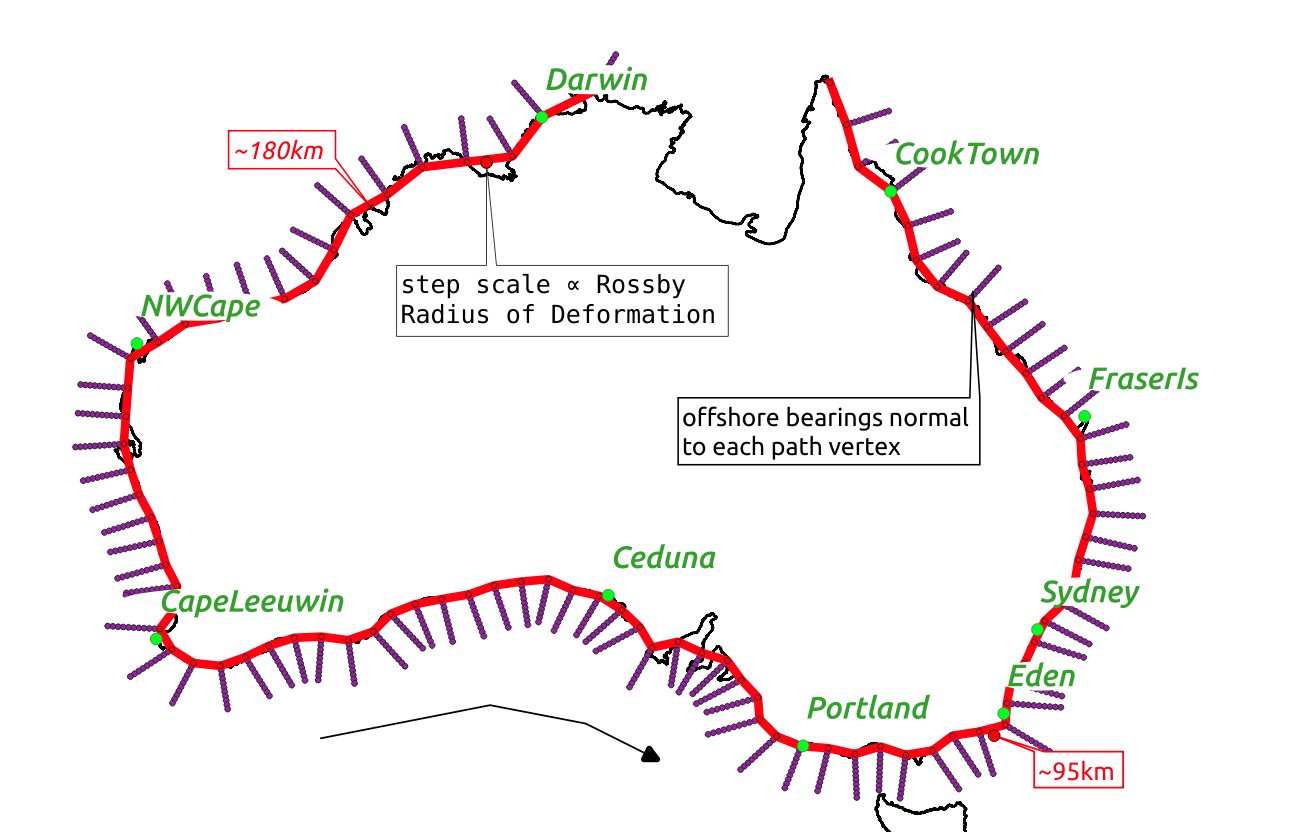
\includegraphics[width=\textwidth]{figures/maps/map_overview.png}
    \end{column}

    \begin{column}{0.5\textwidth}
        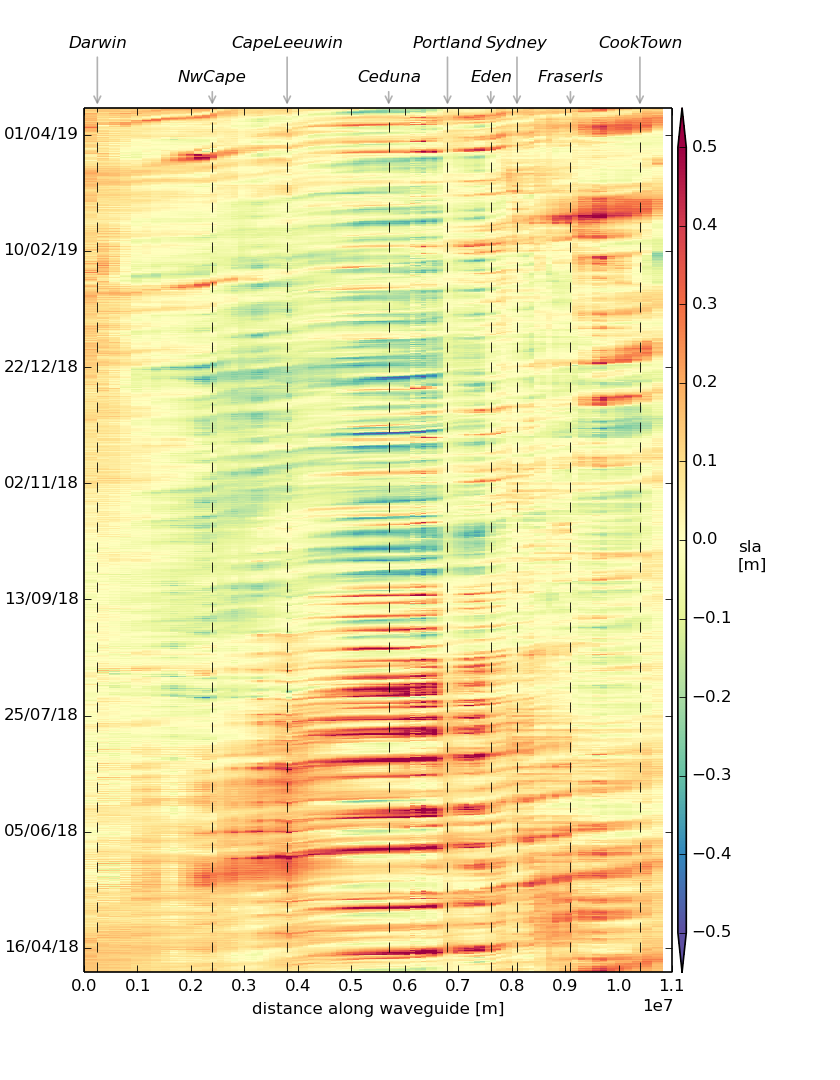
\includegraphics[width=\textwidth]{figures/plots/concat_sla_day0_full.png}
    \end{column}
\end{columns}
\end{frame}
%-----------------------------------------
\begin{frame}
\frametitle{How long is that path?}
    quantitative comparison of celerity
    resolution explicit\\
    but not model dependant
    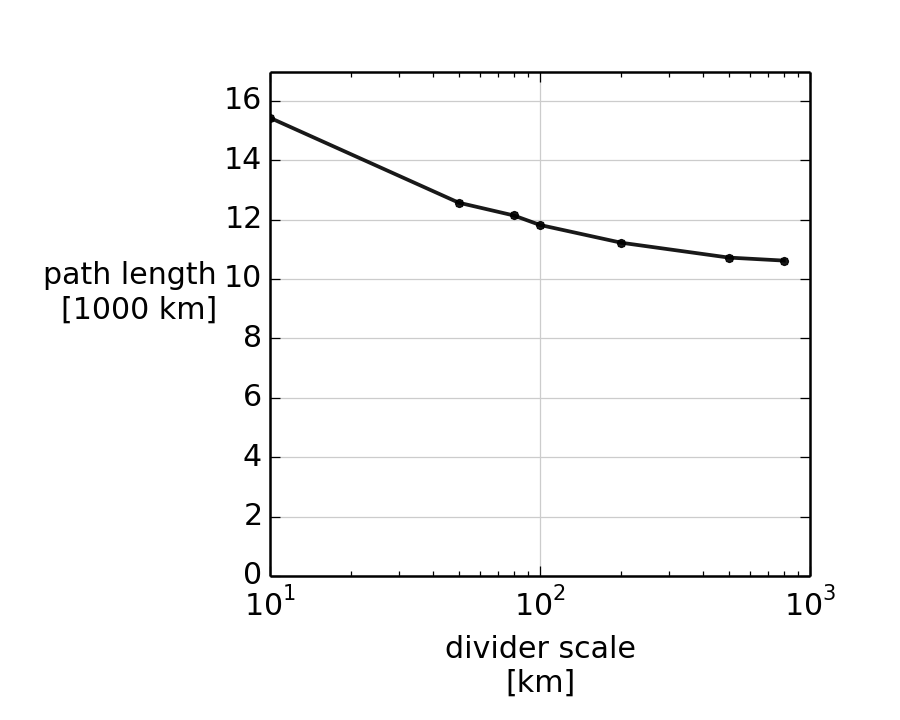
\includegraphics[height=0.6\textheight]{figures/plots/mandelbrot_lengths.png}
\end{frame}
%-----------------------------------------
\begin{frame}
\frametitle{Tides, double counting and adjustments}
ensuring tidal component is fit-for-purpose\\
blunt allocation of constituent cause as "non astromical"\\
conceptual barriers in operations\\
\vfill{}
    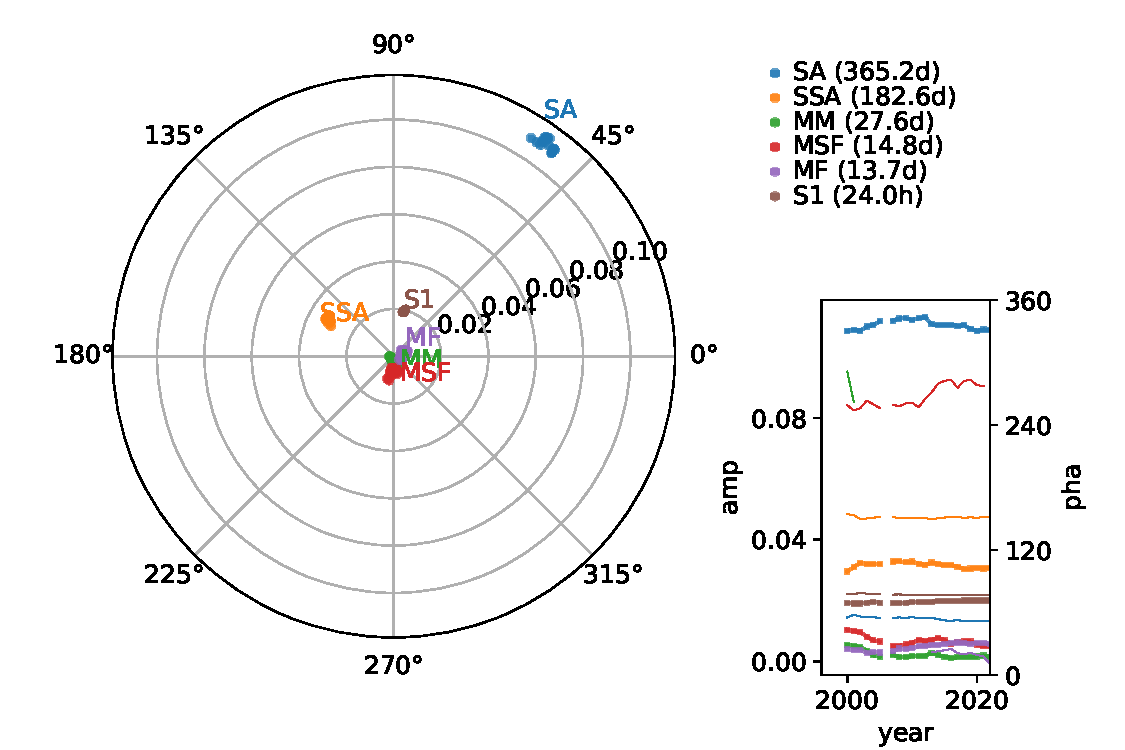
\includegraphics[width=0.45\textwidth]{figures/plots/complex_62290.pdf}
    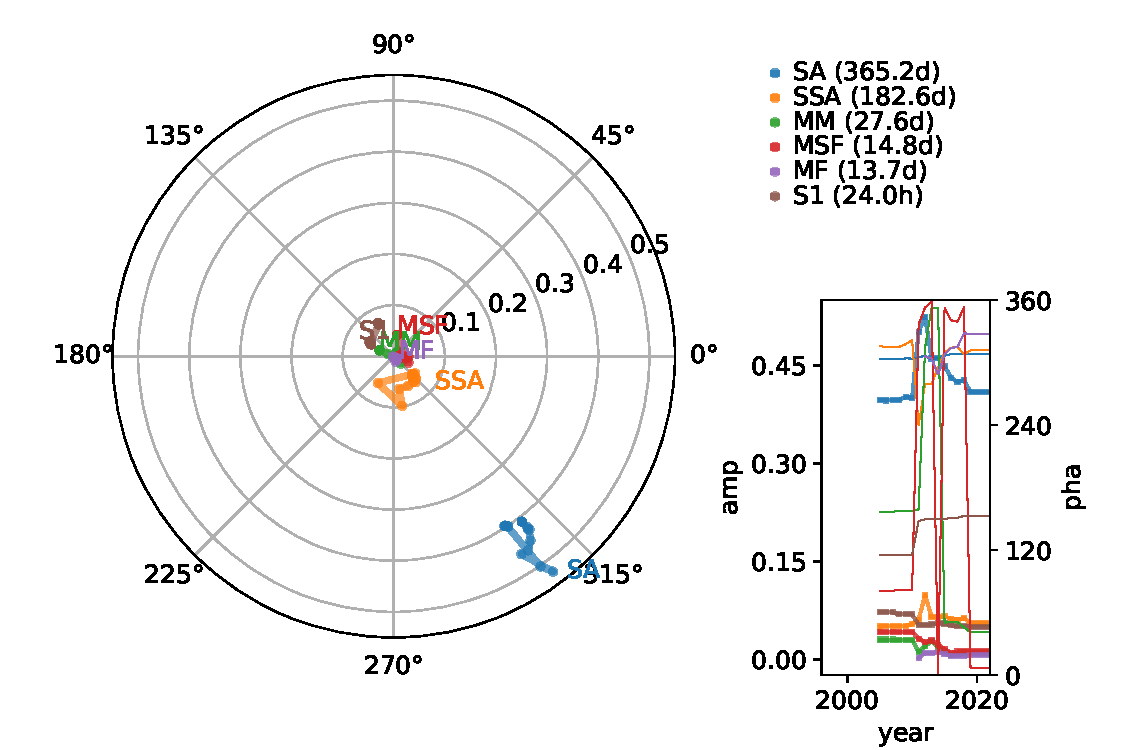
\includegraphics[width=0.45\textwidth]{figures/plots/complex_63540.pdf}
\end{frame}

